\documentclass[tikz,border=10pt]{standalone}
\usepackage{amsmath,amssymb}
\usetikzlibrary{calc,arrows.meta}

\begin{document}
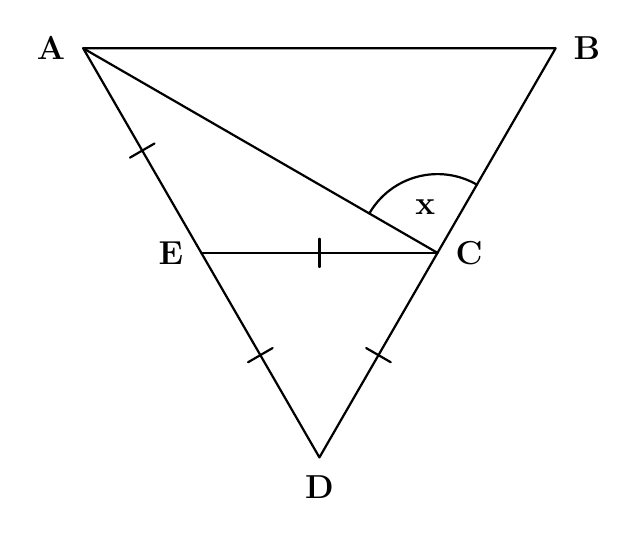
\begin{tikzpicture}[>=latex, line cap=round, line join=round]
  % Coordinates
  \coordinate (D) at (0, 0);
  \coordinate (E) at (-1.5, 2.598);
  \coordinate (C) at (1.5, 2.598);
  \coordinate (A) at (-3.0, 5.196);
  \coordinate (B) at (3.0, 5.196);

  % Outer triangle and segments
  \draw[thick] (A) -- (B) -- (D) -- cycle;
  \draw[thick] (E) -- (C);
  \draw[thick] (A) -- (C);

  % Tick marks function: length 0.35 cm
  % AE tick (at midpoint of AE, angle 120, perpendicular 30)
  \draw[thick] ($($(A)!0.5!(E)$) + (30:0.18)$) -- ($($(A)!0.5!(E)$) + (210:0.18)$);

  % ED tick (at midpoint of ED, angle 120, perpendicular 30)
  \draw[thick] ($($(E)!0.5!(D)$) + (30:0.18)$) -- ($($(E)!0.5!(D)$) + (210:0.18)$);

  % EC tick (at midpoint of EC, angle 0, perpendicular 90)
  \draw[thick] ($($(E)!0.5!(C)$) + (90:0.18)$) -- ($($(E)!0.5!(C)$) + (270:0.18)$);

  % DC tick (at midpoint of DC, angle 60, perpendicular 150)
  \draw[thick] ($($(D)!0.5!(C)$) + (150:0.18)$) -- ($($(D)!0.5!(C)$) + (330:0.18)$);

  % Angle arc for x (from CB at 60 deg to CA at 150 deg)
  \draw[thick] ($(C) + (60:1.0)$) arc (60:150:1.0);
  \node at ($(C) + (105:0.6)$) {\large $\mathbf{x}$};

  % Vertex labels
  \node[left=3pt] at (A) {\large $\mathbf{A}$};
  \node[right=3pt] at (B) {\large $\mathbf{B}$};
  \node[left=3pt] at (E) {\large $\mathbf{E}$};
  \node[right=3pt] at (C) {\large $\mathbf{C}$};
  \node[below=3pt] at (D) {\large $\mathbf{D}$};

\end{tikzpicture}
\end{document}
